%% Chapter 3: Agent-Based Model Investigation

\chapter{Agent-Based Model Investigation}
\label{chap:abm}
In this chapter we use ABMs to simulate SMU and WB in a population of agents. As laid out in the theory of Section~\ref{sec:bg:abm}, using ABMs allows us to model interactions between agents over time, enabling us to understand how realistic non-linear network dynamics can play out. By setting up plausible scenarios and interactions, we demonstrate that the standard research methods of Section~\ref{sec:intro:causal} can fail to identify causal effects when network dependencies and the CoMO effect are present. We also showcase how ABMs can be used as a general tool for investigating complex statistical phenomena. The simulation framework, scenarios, and the resulting bias findings are original contributions of this thesis. Methodological tools from the literature are cited where used.

%% Section 3.1: Motivation
\section{Why Use Agent-Based Models?}
\label{sec:abm:motivation}
In traditional statistical analysis with a regression viewpoint we would typically be drawing observations from some theoretical distribution, or maybe using closed-form model equations to derive our results. The approach using ABMs is different in that it looks at modelling through an individual perspective, allowing for specifications at the individual level, instead of at the aggregate level. This is closer to the stochastic-process viewpoint, where simulating Markov chains using transition probabilities is similar to simulating agents using transition rules. The ABM perspective lets us do this in a way that makes coupling and network interactions easy to set up. We can simulate interactions between individual agents directly, and investigate system dynamics through these simulations. For our investigation into SMU--WB research, ABMs thus give a natural framework to work in, as this area is inherently networked, and individual behaviour plausibly depends on peer behaviour.

As outlined in Section~\ref{sec:intro:causal}, empirical research has applied observational studies, longitudinal studies, and randomised controlled trials (RCTs) to investigate the influence of SMU on WB\@. In this chapter, we will focus specifically on cross-sectional ordinary least squares (OLS) and panel fixed effects as examples of observational and longitudinal approaches. We will also simulate an RCT of our own. We are interested in the statistical foundations of this research, and hence the underlying assumptions.

Some examples of plausible scenarios in the SMU--WB question are scenarios where:
\begin{itemize}
    \item Peer behaviour has an influence on individual behaviour
    \item The WB of an individual depends on relative comparisons with peers
    \item Network effects create feedback loops of influence
\end{itemize}

Whether various study types are still useful for making causal claims in these scenarios can be hard to answer with real data, as we do not know the true parameters or form of the data-generating mechanism. The advantage of ABMs is that they allow us to specify the complete data-generating process (DGP) with known causal effects and effect sizes, with full control over the complexity of the process. Having defined such a process, we can generate synthetic data, apply various research approaches to estimate effects on this synthetic data, and compare estimated effects with true effects. Hence, this approach allows us to investigate the bias of different methods, given varying underlying real worlds. This will be our starting point for investigating what models might be most suitable for estimating the causal effect of SMU on WB\@.

%% Section 3.2: The Simulation Model
\section{The Simulation Model}
\label{sec:abm:model}
The simulations used for the investigation are run in an ABM framework we implement in Python. The framework allows for simulation of a population of $n$ agents over $T$ discrete time steps (days). The agents have stored state variables, learning rules, and update rules for updating their SMU and WB\@. We allow the agents to affect each other through a given network structure. The main text covers the simulations showing how network effects make cross-sectional surveys, panel studies with fixed effects, and RCTs unreliable. Section~\ref{sec:abm:simpsons} further builds on this framework to run a more sophisticated simulation. Numerical settings for all scenarios are collected in Appendix~\ref{app:code:abm}.

\subsection{Agent Attributes and Initialisation}
\label{sec:abm:attributes}
We need to initialise $n$ agents with attributes for their SMU and WB, along with the parameters controlling how these evolve over time. The goal of the initialisation is to create a realistic population with agents having sufficiently heterogeneous SMU and WB with differences in day-to-day variability, all in realistic ranges. We do this by drawing initial values and parameters from prior distributions that reflect semi-realistic ranges. Thus, we ensure that our population of agents is given a reasonable starting point before we start the simulation.

We have two main attributes of interest in our simulations: social media use and well-being. For each agent $i$ and each time $t$ we let these be captured by the variables:

\begin{description}
    \item[Social media use] $s_{it} \in [0, 16]$
    \item[Well-being] $y_{it} \in [0, 10]$
\end{description}

Social media use is measured in hours per day, and bounded to reflect realistic use. Well-being is bounded to $[0, 10]$, an assumed standardised well-being score of interest. An example would be the score from a question using Cantril's ladder, as in \textcite[p.~22]{Cantril1965}.

Each agent is also initialised with four mutable parameters that can be updated by the learning rules. These are:
\begin{itemize}
    \item $\mu^s_i$: ``target'' SMU level (baseline around which actual values fluctuate)
    \item $\sigma^s_i$: variability in SMU
    \item $\mu^y_i$: baseline WB
    \item $\sigma^y_i$: variability in WB
\end{itemize}

We initialise agents by drawing from prior distributions for these parameters. We set the prior distributions to illustrative values. These are set to be broadly consistent with reported SMU and WB levels in the literature \parencite{Twenge2018, Valkenburg2022}. The priors are $\mu^y \sim \N(6.0, 1.0^2)$ for baseline WB, $\mu^s \sim \N(3.0, 0.2^2)$ for target SMU, $\sigma^y \sim \N(1.0, 0.1^2)$ for variability in WB, and $\sigma^s \sim \N(0.2, 0.1^2)$ for variability in SMU\@. We clip the sampled values to keep them in realistic ranges. See Appendix~\ref{app:code:abm} for the details on the clipping bounds.

After this, we initialise the SMU and WB attributes by drawing from each agent's personal priors:
\begin{align}
y_{i0} &= \text{clip}\left(\N(\mu^y_i, \sigma^y_i), 0, 10\right) \\
s_{i0} &= \text{clip}\left(\N(\mu^s_i, \sigma^s_i), 0, 16\right)
\end{align}

\subsection{Network Structure}
\label{sec:abm:network}
We need to define which agents are connected in a network, and are hence allowed to influence each other. For our simulations we want to let each agent be connected to a subset of all the other agents, which we will call its ``neighbours''. We do this through a network structure represented by an adjacency matrix. Such a matrix is a compact way to encode all agent connections, and gives us a way to efficiently compute neighbour-weighted averages (such as the CoMO mechanism) for our simulations.

In Figure~\ref{fig:network_generation_example} we show an example of what such a network could look like with a small number of agents. We provide theoretical background on networks and adjacency matrices in Section~\ref{sec:bg:networks}.

\begin{figure}[htbp]
    \centering
    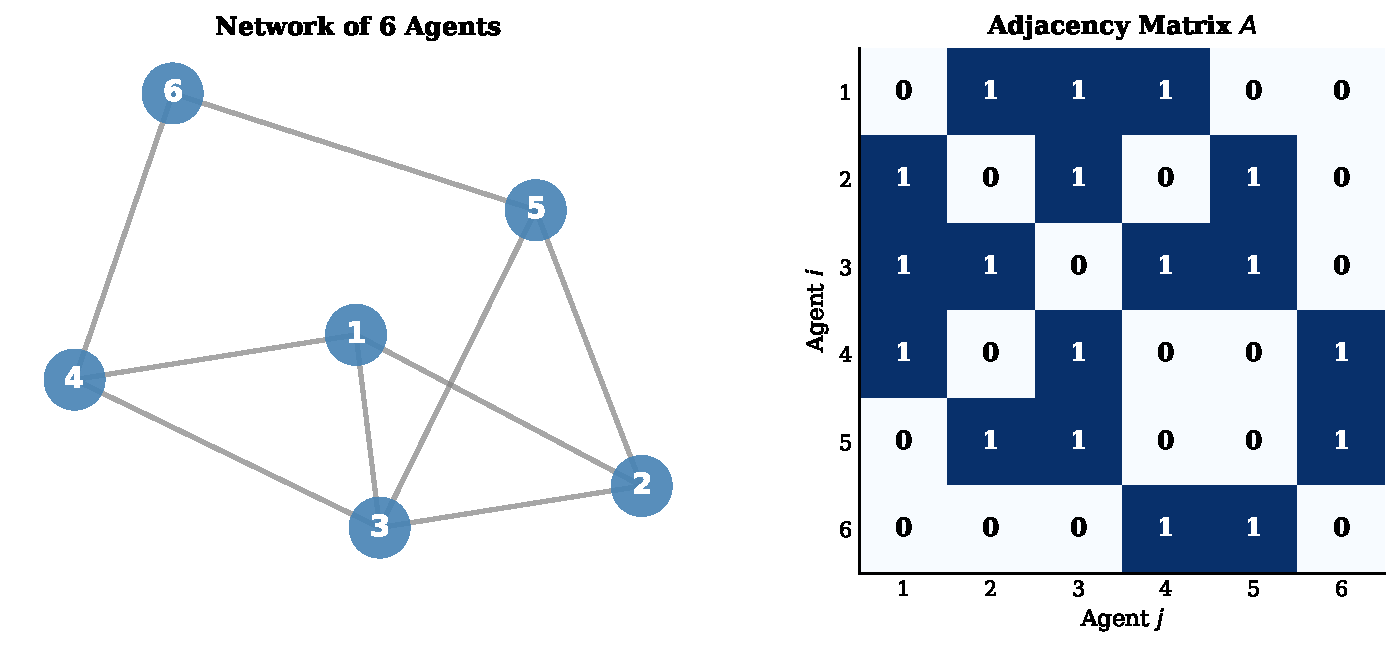
\includegraphics[width=\textwidth]{figures/network_example_chapter_3.pdf}
    \caption[Example network with six agents and corresponding adjacency matrix]{Example of a network with six agents (left) and the corresponding adjacency matrix (right). Nodes represent agents, and edges represent connections. The matrix encodes the network by entries equal to $1$ in each position $(i,j)$ where agent $i$ is connected to agent $j$, with $0$ indicating no connection. Note that this matrix is not normalised.}
    \label{fig:network_generation_example}
\end{figure}

For our population of $n$ agents we need to keep track of who is connected to whom, and we do this by building an adjacency matrix $\mat{G}$ whose element $G_{ij}$ encodes whether agent $i$ is connected to agent $j$. This encoding lets us efficiently compute neighbour-weighted averages such as the CoMO term.

Formally, we let the agent with index $i$ have a set of neighbours $N_i \subseteq \{1, 2, \ldots, n\}$ (assumed to be non-empty), and let $|N_i|$ denote its cardinality. We then define the network structure by the row-normalised adjacency matrix $\mat{G} \in \RR^{n \times n}$ where $G_{ij} = \frac{1}{|N_i|}$ if $j \in N_i$ (i.e., agent $j$ is a neighbour of agent $i$), and $G_{ij} = 0$ otherwise. Due to the row normalisation, $\sum_j G_{ij} = 1$ as all agents have at least one neighbour. With this definition, for any vector $\vect{x} = {(x_1, \ldots, x_n)}^\top$ we have ${(\mat{G}\vect{x})}_i = \frac{1}{|N_i|} \sum_{j \in N_i} x_j$, so $\mat{G}\vect{x}$ returns the vector of all neighbour-weighted averages in a single operation.

The adjacency matrix, along with the CoMO mechanism (see Section~\ref{sec:abm:como}), is used to introduce network effects into our model. When $G_{ij} > 0$, agent $j$ can influence agent $i$. For simplicity, we let all neighbours be equally close in terms of influencing each other.

For the results in this chapter, we construct the network using an Erd\H{o}s--R\'enyi random graph with connection probability $p = 0.1$ \parencite{ErdosRenyi1959, Gilbert1959}. The Erd\H{o}s--R\'enyi-based adjacency matrix is constructed by considering each possible connection between two agents independently. For each such possible connection (pair of agents $i$ and $j$), we create an undirected edge between the two agents with probability $p$, meaning that we have both $i \in N_j$ and $j \in N_i$. The result is a symmetric, unweighted adjacency matrix with $(n-1)p$ as the expected number of neighbours for each agent. For our simulations with $n = 100$ agents and $p = 0.1$ this gives an average of $9.9$ neighbours for each agent; for $n = 500$ it gives approximately $49.9$. After this, we row-normalise and retrieve the finalised adjacency matrix $\mat{G}$.


\subsection{The CoMO Mechanism}
\label{sec:abm:como}
In our simulations we include the CoMO mechanism of \textcite[Eqs.~1--2]{DahlFoldnesGronneberg2024} through the network-structured variant motivated in Section~\ref{sec:bg:social_comparison}, to capture the network effects of social comparison. The mechanism captures the potential of being ``left out'' of activity on social media to be costly. When friends have higher SMU, an individual loses out on social context and shared experiences, incurring a cost.

To formalise this for each agent $i$ at time $t$, we define their CoMO to be the positive gap between their own SMU and the average SMU of a reference group:

\begin{equation}
    c_{it} = \max\left(0, s_{i,t-1}^{\text{ref}} - s_{i,t-1}\right)
    \label{eq:como_main}
\end{equation}

For the results in this chapter, $s_{i,t-1}^{\text{ref}}$ will either be the population mean $\bar{s}_{t-1}$ or, when using an adjacency matrix, the adjacency-weighted neighbour mean ${(\mat{G}\vect{s}_{t-1})}_i = \sum_j G_{ij} s_{j,t-1}$. However, the mechanism allows for any reference group.

The CoMO mechanism introduces a cost to agents with an SMU smaller than the average in the reference group, and hence introduces network effects through peer comparison. In Chapter~\ref{chap:model}, we will provide a more thorough discussion of the CoMO mechanism.

\subsection{Update Rules}
\label{sec:abm:smu_dynamics}
Throughout the simulation, the agent's SMU should be evolving, and we need to specify how this evolution works. Our goal is to create semi-realistic behaviour in our agents, where each agent has habitual usage levels that they tend towards, but where daily use fluctuates. For example, an agent who typically uses social media for three hours might on some days use it for two hours or four hours, but a use of $10$ hours on any day should be extremely unlikely for this agent. We will later specify learning rules to let agents adapt to their environment.

We implement this type of behaviour through a mean-reverting first-order autoregressive (AR(1)) process. In an AR(1) process, we let each value of the process depend on the previous value and some noise. For a process with value $X_t$ at time $t$, $X_t = \phi X_{t-1} + \varepsilon_t$, where $\phi$ is called the persistence parameter and $\varepsilon_t$ is random noise. When $|\phi| < 1$, we say that the process is stationary, and we get a mean-reverting dynamic \parencite[Sec.~3.4, p.~53]{Hamilton1994}.

In our simulations we use such a mean-reverting AR(1) process where each agent's SMU fluctuates around their personal target level $\mu^s_i$. We write the update as:

\begin{equation}
    s_{it} = \phi \cdot s_{i,t-1} + (1 - \phi) \mu^s_i + \varepsilon^s_{it}, \quad \varepsilon^s_{it} \sim \N(0, {(\sigma^s_i)}^2)
    \label{eq:smu_ar1}
\end{equation}
Here, $\phi \in [0, 1)$ controls how quickly the agents revert to their target, and ensures the magnitude of changes in behaviour stays reasonable between each time step. In this way, agents are allowed to change behaviour, but still remain close to stable habitual behaviour of the past. The term $\mu^s_i$ pulls the agent towards its target SMU level. $\varepsilon^s_{it}$ is an error term that makes the process stochastic. For simplicity, we reuse the agent-specific scale $\sigma^s_i$ from initialisation rather than introducing a separate noise parameter. The target is updated through the learning rule, which allows the agents to adapt without extreme changes. We also clip the SMU values to $[0, 16]$ hours per day to ensure realistic values.

As with SMU, we need to define how agents' WB is updated throughout the simulation. We want each agent to have daily variation around a more stable trend. Well-being should be allowed to vary, as some agents are naturally happier than others, but we do not want overly large jumps from day to day. We also want the WB to be influenced directly by SMU and the CoMO effect. Each agent's use of social media should influence WB, and peer comparison should influence WB for agents below the average when the CoMO mechanism is active.

Combining these, we use the following update rule for the WB of agent $i$ at time $t$:

\begin{equation}
    y_{it} = \mu^y_i + \gamma_1 s_{it} + \gamma_2 \cdot c_{it} + \varepsilon^y_{it}, \quad \varepsilon^y_{it} \sim \N(0, {(\sigma^y_i)}^2)
    \label{eq:wb_basic}
\end{equation}
Here, $\mu^y_i$ is agent $i$'s baseline WB and $\varepsilon^y_{it}$ is the stochastic error term, while $\gamma_1$ and $\gamma_2$ measure the influence of SMU and CoMO on WB, respectively. Unlike with SMU, we model WB without persistence. We do this for simplicity, and because our interest is mainly in the contemporaneous effects of SMU and CoMO on WB\@.

Section~\ref{sec:abm:simpsons} extends this update rule to add delayed effects.

\subsection{Learning Rules}
\label{sec:abm:learning}
To make simulations more realistic, we implement learning to let agents adapt their behaviour based on the past. In real life, people generally adjust their behaviour based on experience. Thus, if an agent has a high SMU, leading to a low WB, we want them to be able to notice and change their behaviour accordingly. Similarly, if increasing SMU leads to increasing WB, agents should be given a way to notice this and adapt. This learning is crucial for the simulation, as it allows emergent behaviour to occur as agents adapt to their social environment.

In general we can allow the learning to target all attributes of the agent. For the simulations presented here, we let agents learn by updating their target SMU, $\mu^s_i$. Thus, the update also changes the magnitude of the influence on WB through SMU (and variables using SMU).

Agents update their target SMU using regression-based learning, as a way to move towards higher WB\@. This lets agents remember how their last days have been, what they did on those days, and update their behaviour based on any recent trends. For each agent we store a rolling window of the $W$ most recent $(s_{it}, y_{it})$ pairs. $W$ should not be very large, as learning based on more than just a few recent days is unrealistic. We estimate the slope of WB regressed on SMU on these pairs using OLS:
\begin{equation}
    \hat{\beta}_{it} = \frac{\sum_{\tau=1}^{W}(s_{i,t-\tau} - \bar{s}_{iW})(y_{i,t-\tau} - \bar{y}_{iW})}{\sum_{\tau=1}^{W}{(s_{i,t-\tau} - \bar{s}_{iW})}^2}
\end{equation}

Then, we update the target as follows:
\begin{equation}
    \mu^s_i \leftarrow \mu^s_i + \eta \cdot \text{clip}(\hat{\beta}_{it}, -5, 5)
\end{equation}

Here, $\eta$ is the learning rate, and we clip the estimated slope to avoid extreme values.

Thus, at each time $t$, each agent estimates the relationship between SMU and WB based on their own experience over the last few days, and moves their baseline behaviour slightly in the direction of increasing their own WB\@. This implementation of learning would be hard to model using standard statistical methods, but using ABMs makes this feasible.


\subsection{Design of Three Simulation Scenarios}
\label{sec:abm:dynamics}
For the results in this chapter, we simulate three different scenarios:

\begin{itemize}
    \item \textbf{Reference:} Baseline where all study types should recover the correct parameters. No network effects, neither CoMO nor adjacency.
    \item \textbf{CoMO:} Same as reference, but with the addition of population-mean-based CoMO with $\gamma_2 = -0.4$. No adjacency.
    \item \textbf{Network \& CoMO:} Same as reference, but with adjacency-weighted CoMO (still $\gamma_2 = -0.4$).
\end{itemize}

For each scenario, the simulation flow is as follows:

\begin{enumerate}
  \item Initialise $n$ agents with attributes (see Section~\ref{sec:abm:attributes}).
  \item For each time step $t = 1, \ldots, T$:
  \begin{enumerate}
    \item Compute CoMO\@.
    \item Update SMU and WB\@.
    \item Apply learning and update attributes.
  \end{enumerate}
\end{enumerate}

We simulate for $T = 500$ time steps, discard the first $B = 100$ time steps as burn-in, and store the results from the other time periods. In the case of the RCTs, the simulations are altered slightly (see Section~\ref{sec:abm:methods}). After simulating, we can apply the various research methods whose performance we wish to investigate. For an overview of the parameters used in the scenarios, see Table~\ref{tab:abm_main_params}.

\begin{table}[htbp]
\centering
\caption[Main parameter values used in simulations]{Main parameter values used in simulations.}
\label{tab:abm_main_params}
\begin{tabular}{llc}
\toprule
Parameter & Description & Value \\
\midrule
$n$ & Number of agents & 100 (500 for RCT) \\
$T$ & Number of days & 500 \\
$B$ & Burn-in period & 100 \\
$\phi$ & SMU persistence & 0.5 \\
$\gamma_1$ & SMU$\to$WB coefficient & $-0.5$ \\
$\gamma_2$ & CoMO$\to$WB coefficient & $-0.4$ \\
$\eta$ & Learning rate & 0.05 \\
$W$ & Learning window & 10 \\
\bottomrule
\end{tabular}
\end{table}

We note that the target estimand investigated in this chapter is the direct effect of own SMU on WB, with corresponding parameter $\gamma_1$. This scoping thus does not emphasise total effects. This simplification suffices for what we want to illustrate. The DGPs used are also illustrative, and not empirically calibrated. We use negative values for $\gamma_1$ and $\gamma_2$ for concreteness, but emphasise that the bias mechanisms found are due to the network effects. Thus, sign reversal would not change the conclusion. The simulations are therefore best interpreted as showing what \emph{can} happen in plausible networked worlds, not what \emph{does} happen in the SMU--WB literature.

%% Section 3.3: Implementation of Research Methods in Simulations
\section{Implementation of Research Methods in Simulations}
\label{sec:abm:methods}
To test our simulation results we implement three research methods that have been commonly used in the SMU--WB literature. For an explanation of how each method works and the assumptions they make, see Section~\ref{sec:intro:causal}. This section describes how each method is applied to the simulated data as a way to investigate the bias introduced by the network effects of the CoMO mechanism and adjacency implementation.

For the cross-sectional OLS (see Section~\ref{sec:intro:cross_sectional}), we need to use the output of the simulation at a single time step. We choose to use the last time step of the simulation, and hence regress WB on SMU across all $n$ agents at this time step. This gives an estimate of the cross-sectional association between SMU and WB at that time, which we interpret as an estimate of $\gamma_1$. The cross-sectional OLS estimator gives the answer that the approach most commonly used in empirical research (giving people a one-time survey asking about their SMU and WB) would give.

When it comes to the panel fixed effects estimation (described in Section~\ref{sec:intro:panel}), we use the data from the simulation after the burn-in period. Hence, we have $T - B = 400$ observations per agent. We first demean the data for each agent by subtracting their respective individual mean from their observations. Afterwards, we estimate the association between SMU and WB using the demeaned data, getting an estimate for $\gamma_1$. This procedure allows us to isolate within-agent variation over time, as it removes all time-invariant agent attributes from the estimation procedure.

To perform a simulated RCT (see Section~\ref{sec:intro:rct} for theory on RCTs), we need to decide on what intervention to simulate. We decide on the following treatment as an illustrative intervention. After the burn-in period, we assign $20\%$ of agents randomly to the treatment. The other $80\%$ of agents receive no treatment. The treated agents are capped in how much SMU they can have per day, to one hour per day. This cap is in effect for the rest of the simulation. The other agents (the ones in the control group) continue as normal, learning and modifying their behaviour as described in previous sections.

To be able to compare the treatment effect resulting from this simulation, we use the scaled estimator from Equation~\eqref{eq:rct_scaled}. This divides the difference in mean WB between the two groups by the difference in their mean SMU\@. Performing this scaling converts the treatment effect to a unit comparable to $\gamma_1$, which allows us to directly compare the estimated effect from the RCT with the estimates from cross-sectional OLS and the panel data with fixed effects. As in the cross-sectional OLS, we use the observations from the final time step for our RCT estimates.

The three methods are different in their implementations, which leads to large differences in their effective sample size (ESS). Cross-sectional OLS uses the $n$ observations at the final time step, and thus has an effective sample size of $n = 100$. The panel fixed effects use the temporal structure to draw on $n \times (T - B) = 40{,}000$ observations, giving them a substantially higher ESS than the other methods, though serial correlation in the AR(1) SMU process means the effective information is somewhat less than $40{,}000$ independent samples. The RCT, on the other hand, with its estimate based on the difference between the treated and control groups, achieves an effective sample size dominated by the smaller group. With $n = 100$ and $20\%$ treated, this leads to an ESS well below $100$, far lower than the other two.

To make the methods more comparable, we adjust the sample size for the RCT simulations by setting $n = 500$. With $20\%$ being assigned to the treatment, this brings the RCT's ESS closer to that of cross-sectional OLS, making noise from variation due to sample size more similar across the two methods. We choose not to make any adjustments to the panel fixed effects, as we consider the larger ESS an inherent advantage of the method. Making this adjustment, we can more easily interpret differences in bias as coming from network effects violating assumptions, and not just differences in sample size. We note that, as $p = 0.1$ is fixed, the increase in $n$ also increases the expected degree. Thus, this adjustment partly conflates method and density effects. Future work could perform a more careful analysis.

%% Section 3.4: Simulation Results
\section{Simulation Results}
\label{sec:abm:results}
We run and report results from simulations of the three scenarios. We run $M = 250$ simulations for each scenario and report Monte Carlo verification of bias estimates across these runs. We also plot the distributions of estimates to verify bias.

\subsection{Reference Scenario}
\label{sec:abm:reference}
Before investigating how the network effects introduced by CoMO and adjacency affect the results of the three research methods, we verify that the methods correctly recover the direct effect of SMU on WB, $\gamma_1 = -0.5$, when these mechanisms are absent. Hence, in the reference scenario we remove the CoMO effect on WB by setting $\gamma_2 = 0$ in Equation~\eqref{eq:wb_basic}. This yields the WB update equation:
\begin{equation}
    y_{it} = \mu^y_i + \gamma_1 s_{it} + \varepsilon^y_{it} = \mu^y_i - 0.5 \cdot s_{it} + \varepsilon^y_{it}
    \label{eq:wb_reference}
\end{equation}
The result is a simple DGP where the WB of an agent only depends on the agent's own SMU through $\gamma_1$, which the three research methods should be able to correctly recover.

\begin{table}[htbp]
\centering
\caption[Mean estimates of direct effect in the reference scenario]{Mean estimates of direct effect in the reference scenario across $M = 250$ Monte Carlo replications. True effect: $\gamma_1 = -0.5$.}
\label{tab:abm_reference}
\begin{tabular}{lcc}
\toprule
Method & Mean Estimate & Relative Bias (\%) \\
\midrule
Cross-sectional OLS & $-0.489$ & $2.3\%$ \\
Panel Fixed Effects & $-0.500$ & $0.1\%$ \\
RCT & $-0.487$ & $2.7\%$ \\
\bottomrule
\end{tabular}
\end{table}

The results for the simulations in the reference scenario are reported in Table~\ref{tab:abm_reference}. They show that all three methods recover a good estimate of the true effect of SMU on WB\@. This is as expected, as the reference DGP satisfies the assumptions needed for the methods to give unbiased results. In particular, we see that cross-sectional OLS gives a mean estimate of $-0.489$, panel fixed effects gives $-0.500$, and the RCT gives $-0.487$. All three estimates are close to the true value $\gamma_1 = -0.5$, confirming that our simulations and estimation procedures are implemented correctly.

\begin{figure}[htbp]
    \centering
    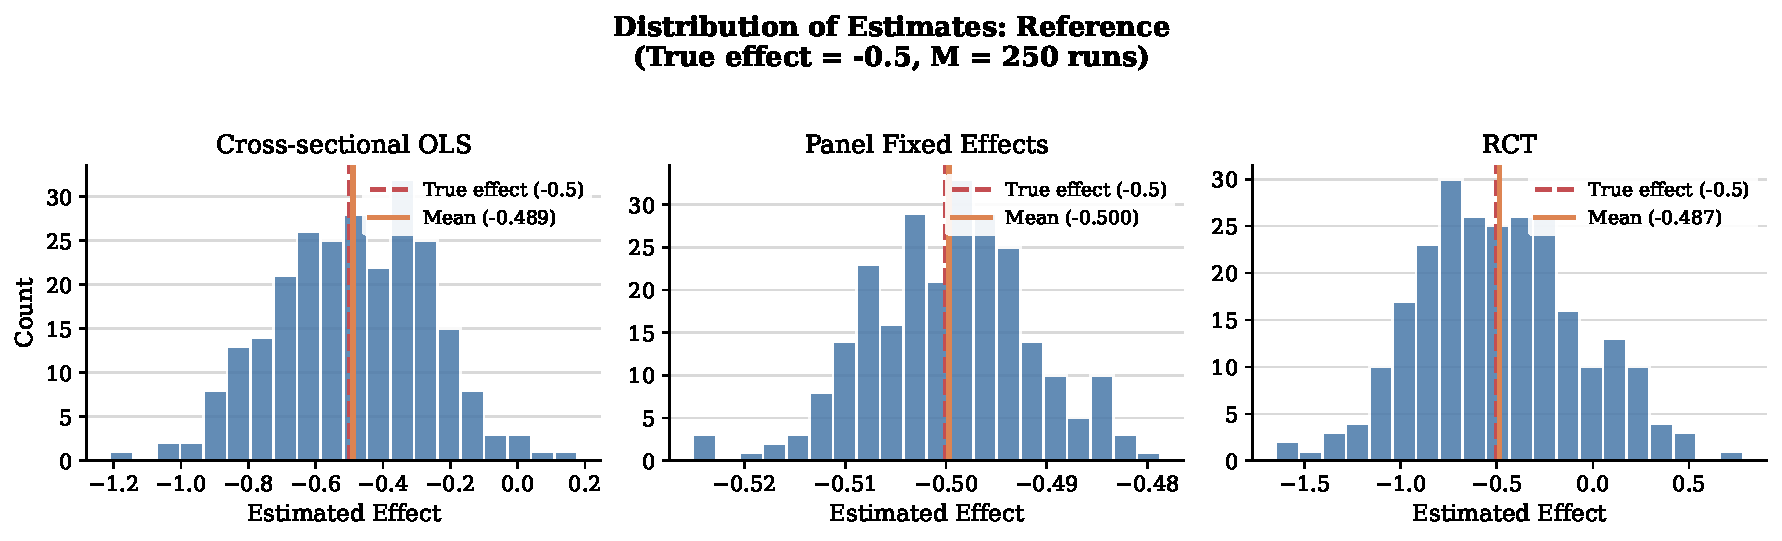
\includegraphics[width=\textwidth]{figures/abm_histogram_reference.pdf}
    \caption[Distribution of estimates for the reference scenario]{Distribution of simulation estimates for the reference scenario. All three methods correctly cluster around the true effect ($\gamma_1 = -0.5$, shown as vertical dashed line) when CoMO and agent adjacency are absent.}
    \label{fig:abm_histogram_reference}
\end{figure}

We also plot the distribution of the estimated values in Figure~\ref{fig:abm_histogram_reference}, where we see that the values are spread evenly around the true value. We note that the variation of the panel fixed effects is substantially smaller than that of the cross-sectional OLS and RCT\@. The RCT has slightly higher variation than OLS, despite comparable ESS\@. This is expected due to the additional SMU components in the scaled estimator (Equation~\eqref{eq:rct_scaled}) contributing some variance. The reference scenario establishes a baseline for comparison of the bias introduced by the CoMO and adjacency mechanisms in the other scenarios.

\subsection{CoMO Scenario}

In the second simulation we include the CoMO variable. With $\gamma_2 = -0.4$ this gives the following WB update equation:

\begin{equation}
    y_{it} = \mu^y_i + \gamma_1 s_{it} + \gamma_2 \cdot c_{it} + \varepsilon^y_{it}
     = \mu^y_i - 0.5 \cdot s_{it} - 0.4 \cdot c_{it} + \varepsilon^y_{it}
    \label{eq:wb_como}
\end{equation}

In this scenario the $c_{it} = \max(0, \bar{s}_{t-1} - s_{i,t-1})$ mechanism uses the population mean $\bar{s}_{t-1}$ as the reference group. This introduces network effects to the simulation through the peer comparison in the CoMO term. As the three research methods we are testing do not account for this in their structure, we expect them to yield biased results, which is exactly what we find in our simulations (see Table~\ref{tab:abm_como}): cross-sectional OLS gives a mean estimate of $-0.400$ with a bias of $20.1\%$, panel fixed effects yields $-0.391$ with a bias of $21.8\%$, and the RCT estimates $-0.371$ with a bias of $25.9\%$.

\begin{table}[htbp]
\centering
\caption[Mean estimates of direct effect in the CoMO scenario]{Mean estimates of direct effect in the CoMO scenario across $M = 250$ Monte Carlo replications. True effect: $\gamma_1 = -0.5$.}
\label{tab:abm_como}
\begin{tabular}{lcc}
\toprule
Method & Mean Estimate & Relative Bias (\%) \\
\midrule
Cross-sectional OLS & $-0.400$ & $20.1\%$ \\
Panel Fixed Effects & $-0.391$ & $21.8\%$ \\
RCT & $-0.371$ & $25.9\%$ \\
\bottomrule
\end{tabular}
\end{table}

Figure~\ref{fig:abm_histogram_como} shows the distribution of the estimates together with the true coefficient, showing a clear bias towards zero for all three methods. Hence, our results show that all three methods correctly identify the direction of the effect, but underestimate its magnitude when the CoMO mechanism is present. The bias towards zero is expected: when CoMO is introduced, agents who would otherwise benefit from low SMU are instead also affected negatively through the CoMO mechanism. Methods that do not take CoMO into account will fail to capture all of this negative association. With more negative association among the agents with lower SMU, the slope of the association flattens out, and we see a bias towards zero.

\begin{figure}[htbp]
    \centering
    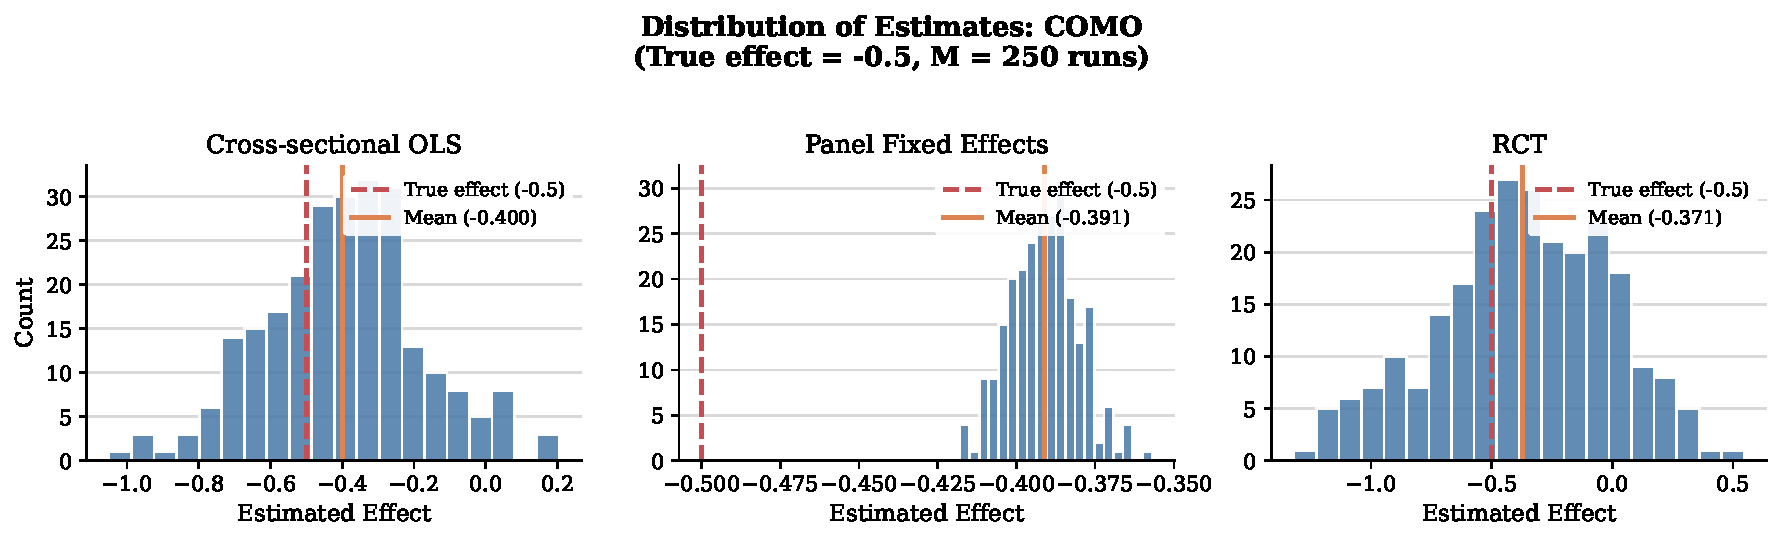
\includegraphics[width=\textwidth]{figures/abm_histogram_como.pdf}
    \caption[Distribution of estimates for the CoMO scenario]{Distribution of simulation estimates for the CoMO scenario. The true effect $\gamma_1 = -0.5$ is marked with a vertical dashed line. All methods show bias towards zero due to peer comparison through CoMO\@. As in the reference case, panel fixed effects has lower variance due to higher ESS.}
    \label{fig:abm_histogram_como}
\end{figure}

\subsection{Network \& CoMO Scenario}

The final scenario introduces both an adjacency matrix $\mat{G}$ and the CoMO mechanism. The adjacency matrix is constructed as an Erd\H{o}s--R\'enyi network with connection probability $p = 0.1$ as described in Section~\ref{sec:abm:network}. Using this matrix, we now calculate CoMO as $c_{it} = \max(0, {(\mat{G}\vect{s}_{t-1})}_i - s_{i,t-1})$ using the adjacency-weighted neighbour mean ${(\mat{G}\vect{s}_{t-1})}_i = \sum_j G_{ij} s_{j,t-1}$. Hence, we introduce local peer comparison, instead of the global comparison of the CoMO scenario.

With the same parameters as we used before, the WB update equation becomes:
\begin{equation}
    y_{it} = \mu^y_i - 0.5 \cdot s_{it} - 0.4 \cdot c_{it} + \varepsilon^y_{it}
    \label{eq:wb_network_como}
\end{equation}

The results are presented in Table~\ref{tab:abm_network_como}, and show the following: cross-sectional OLS yields a mean estimate of $-0.371$ with a bias of $25.7\%$, panel fixed effects produces $-0.391$ with a bias of $21.8\%$, and the RCT gives $-0.341$ with a bias of $31.9\%$.

\begin{table}[htbp]
\centering
\caption[Mean estimates of direct effect in the Network \& CoMO scenario]{Mean estimates of direct effect in the Network \& CoMO scenario across $M = 250$ Monte Carlo replications. True effect: $\gamma_1 = -0.5$.}
\label{tab:abm_network_como}
\begin{tabular}{lcc}
\toprule
Method & Mean Estimate & Relative Bias (\%) \\
\midrule
Cross-sectional OLS & $-0.371$ & $25.7\%$ \\
Panel Fixed Effects & $-0.391$ & $21.8\%$ \\
RCT & $-0.341$ & $31.9\%$ \\
\bottomrule
\end{tabular}
\end{table}

As with the CoMO scenario, we see correct sign estimation, but an underestimation of the effect magnitude. In practice, this means that we underestimate the harmful effects of SMU on WB\@. The RCT shows the largest bias here (under the network-density caveat from Section~\ref{sec:abm:methods}), and the increase in bias from the global to the local comparison is larger for the RCT than for OLS\@. When we change from global peer comparison to local, network effects become stronger. The smaller reference group increases the network influence, while the global comparison averages it out more. Local groups allow for larger magnitude and variation in effects.

\begin{figure}[htbp]
    \centering
    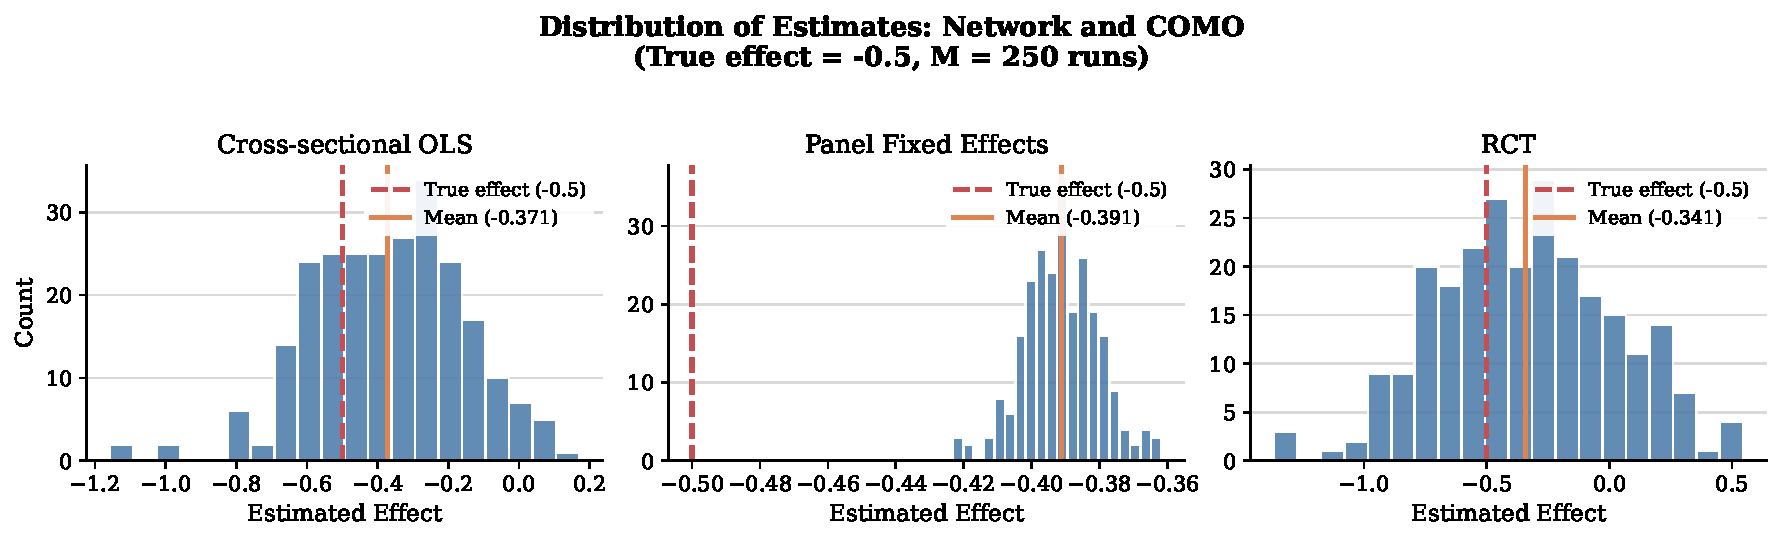
\includegraphics[width=\textwidth]{figures/abm_histogram_network_como.pdf}
    \caption[Distribution of estimates for the Network \& CoMO scenario]{Distribution of simulation estimates for the Network \& CoMO scenario using an Erd\H{o}s--R\'enyi graph with $p = 0.1$. The true effect $\gamma_1 = -0.5$ is marked with a vertical dashed line. All methods show bias towards zero, with the RCT having the largest bias.}
    \label{fig:abm_histogram_network_como}
\end{figure}

\subsection{Summary of Simulation Results}

We present a summary of the results across all three scenarios and research methods in Table~\ref{tab:abm_summary}. The table compares mean effect estimates, absolute bias, and relative bias.

\begin{table}[htbp]
\centering
\caption[Simulation results across all scenarios and methods]{Simulation results across all scenarios and methods. True effect: $\gamma_1 = -0.5$. Results based on $M = 250$ Monte Carlo replications per scenario.}
\label{tab:abm_summary}
\begin{tabular}{llccc}
\toprule
Scenario & Method & Mean & Abs.\ Bias & Rel.\ Bias (\%) \\
\midrule
Reference & Cross-sectional OLS & $-0.489$ & $0.011$ & $2.3\%$ \\
Reference & Panel Fixed Effects & $-0.500$ & $0.000$ & $0.1\%$ \\
Reference & RCT & $-0.487$ & $0.013$ & $2.7\%$ \\
\midrule
CoMO & Cross-sectional OLS & $-0.400$ & $0.100$ & $20.1\%$ \\
CoMO & Panel Fixed Effects & $-0.391$ & $0.109$ & $21.8\%$ \\
CoMO & RCT & $-0.371$ & $0.129$ & $25.9\%$ \\
\midrule
Network \& CoMO & Cross-sectional OLS & $-0.371$ & $0.129$ & $25.7\%$ \\
Network \& CoMO & Panel Fixed Effects & $-0.391$ & $0.109$ & $21.8\%$ \\
Network \& CoMO & RCT & $-0.341$ & $0.159$ & $31.9\%$ \\
\bottomrule
\end{tabular}
\end{table}

The results have some clear takeaways: in the reference scenario, the research methods work as intended, and are all able to capture the true effect of SMU on WB ($\gamma_1 = -0.5$). With $M = 250$ Monte Carlo replications, we observe very low bias for all three methods in the reference. In the CoMO and Network \& CoMO scenarios, all the effect estimates are biased towards zero under the specified DGPs, with the bias ranging from around $20\%$ to $32\%$. The RCT, often perceived as the most robust study type (see Section~\ref{sec:intro:rct}), shows the largest bias in our simulations (although the caveat from Section~\ref{sec:abm:methods} should be noted). This is due to the violation of the SUTVA assumption that its estimation rests on, coming from spillover effects from the treated group. When the agents in the treatment group reduce their SMU, this changes the reference level for the untreated agents, leading to biased estimates.

In Figure~\ref{fig:abm_forest}, we also provide a forest plot summary of the results with confidence bands to give a visualisation of the uncertainty from the Monte Carlo replications. This shows how the cross-sectional OLS and RCT have similar variation due to comparable ESS (with the RCT slightly wider), while the panel fixed effects method yields a much higher ESS, and thus a much lower variation.

\begin{figure}[htbp]
    \centering
    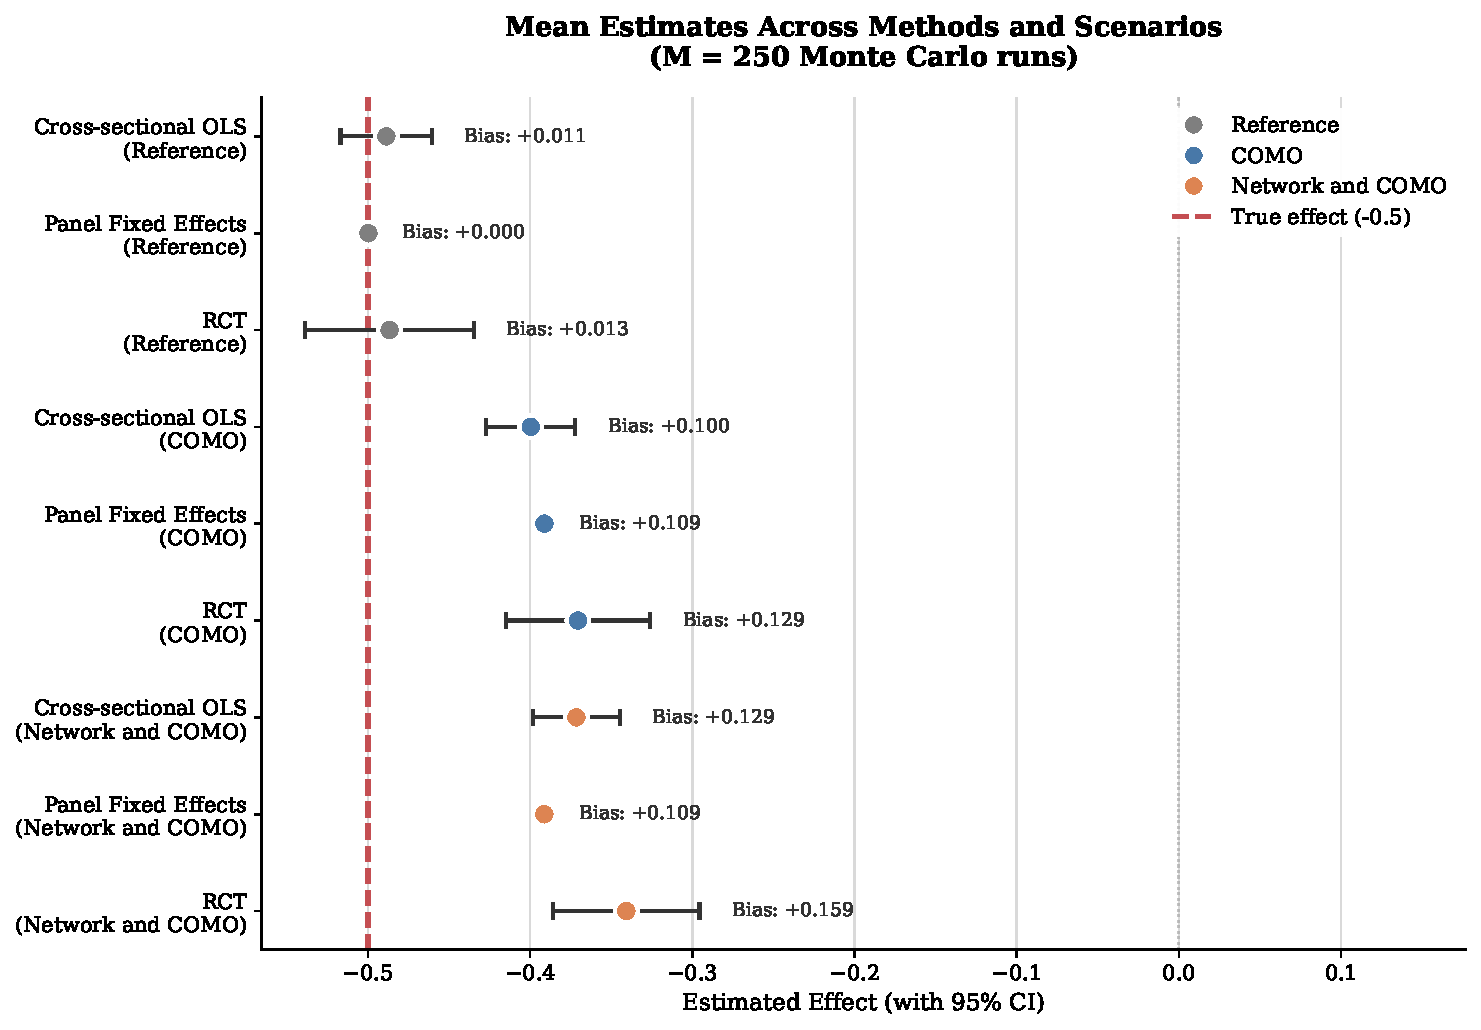
\includegraphics[width=\textwidth]{figures/abm_forest.pdf}
    \caption[Forest plot of mean estimates by method and scenario]{Forest plot of mean estimates for all methods and scenarios. Error bars show the $95\%$ CI of the mean across the Monte Carlo replications. The true effect $\gamma_1 = -0.5$ is marked with a vertical dashed line. All the methods exhibit bias in the non-reference scenarios.}
    \label{fig:abm_forest}
\end{figure}

%% Section 3.5: Demonstration of Simpson's Paradox
\section{Demonstration of Simpson's Paradox}
\label{sec:abm:simpsons}
The ABM framework we have implemented is general and allows for more complex simulations than the ones we have run above. ABMs have been proposed as a tool for simulating complex large-scale systems, including entire national economies \parencite{Farmer2009}. To demonstrate the versatility of the framework and how it can be used to investigate complex statistical phenomena, we use simulations to demonstrate Simpson's Paradox in the SMU--WB case.

In our case, we will demonstrate how, under plausible model assumptions, we can get a scenario where SMU has a negative influence on WB, and increased SMU leads to a decrease in WB on a population level, but where regressing WB on SMU at any given time $t$ will still yield a positive association. This showcases the intricacies involved in the research of the causal effect of SMU on WB\@.

\subsection{Background: What is Simpson's Paradox?}
\label{sec:abm:simpsons:bg}
Simpson's Paradox, first described by \textcite{Simpson1951}, is a phenomenon where a statistical association observed in aggregated data reverses or disappears when the data is partitioned into subgroups. The paradox is not just a statistical curiosity; it can occur in real data and thus has implications for causal inference. We provide an example of a classic version of Simpson's Paradox to explain the phenomenon.

\begin{example}[Classic Simpson's Paradox]
\label{ex:simpsons}
We construct a toy dataset for a study on the effectiveness of a treatment in two hospitals. In Hospital A, mostly severe cases are treated, while in Hospital B there are mostly mild cases:

\begin{center}
\begin{tabular}{lccc}
\toprule
 & Hospital A & Hospital B & Combined \\
\midrule
Treated patients ($n$) & 1{,}000 & 100 & 1{,}100 \\
Treatment success rate & $40\%$ & $90\%$ & $44.5\%$ \\[4pt]
Control patients ($n$) & 100 & 1{,}000 & 1{,}100 \\
Control success rate & $30\%$ & $80\%$ & $75.5\%$ \\
\midrule
Treatment effect & $+10\%$ & $+10\%$ & $-31\%$ \\
\bottomrule
\end{tabular}
\end{center}

Here we have constructed our toy data such that the treatment is beneficial in each hospital separately ($+10\%$ in both), but still appears harmful in total when we aggregate the data ($-31\%$). The effect stems from the unequal allocation between the two hospitals. Hospital A treats more serious cases (low baseline success rates), and contains the majority of treated patients. Hospital B, on the other hand, mostly treats milder cases, but contains most of the control patients. When aggregating, this leads to the treated group being dominated by the harder cases of Hospital A, while the control group contains mostly the easier patients from Hospital B, leading to a reversal of the observed association.
\end{example}

To not be confused by Simpson's Paradox we need to employ careful causal reasoning. The correct analysis of a problem depends on its causal structure. In the language of causal inference: if a hospital is a confounder (with an effect on both treatment assignment and outcomes, as it is in Example~\ref{ex:simpsons}), we need to condition on it. However, if the hospital is a mediator (where the treatment affects the outcome through the hospital choice), we should not. The logic of when to condition and when not to condition to land at the correct causal conclusion is discussed in \textcite[Ch.~6]{Pearl2009}.

There are multiple factors that make Simpson's Paradox a phenomenon that is particularly relevant to SMU--WB research:
\begin{itemize}
    \item \textbf{Aggregation happening over time}: Longitudinal trends and cross-sectional associations calculated at any given time point are not necessarily the same. Thus, it is possible to have a positive association between individual SMU and WB at any given moment (where those feeling better also have higher SMU), while still having increased SMU causing lower WB over time.
    \item \textbf{Network heterogeneity}: Due to network effects, associations within peer groups may be different from associations found at the population level due to homophily \parencite{McPherson2001} and peer influence.
    \item \textbf{Selection effects}: If there are selection effects present, where for example individuals with high SMU differ in some systematic way from those with low SMU, this can confound the relationship between SMU and WB\@.
\end{itemize}

\subsection{Adjusted Simulation Design}
\label{sec:abm:simpsons:design}
To demonstrate Simpson's Paradox, we add another component to our simulation structure, which we will call the \emph{delayed decline} mechanism. We include this mechanism to capture the idea that SMU might lead to short-term reward through entertainment and social connection, but long-term costs through reduced sleep quality and increased social comparison \parencites{Valkenburg2022}[Ch.~5]{Haidt2024}, see also Section~\ref{sec:bg:social_comparison}. An increased strength in the effect of CoMO on WB combined with this mechanism leads to the paradox arising.

The delayed decline mechanism alters the WB update rule by adding a temporal structure to how SMU influences WB\@. This is done through an impulse response function, which is a concept from time series analysis used to describe a system response over time to a one-time shock \parencite[Sec.~1.1, p.~5]{Hamilton1994}. In this way we can implement delayed consequences of SMU into our simulations. For our impulse response function we use a difference-of-exponential kernel, which is commonly used for modelling drug effects with varying onset and decay rates \parencite[Eq.~(9.11), p.~207]{Rosenbaum2016}.

The technical implementation adds these delayed decline terms to WB for each agent $i$ at each time $t$, computed as a sum of difference-of-exponentials weighted by past SMU values:
\begin{equation}
    \Delta y_{it}^{\text{delayed}} = \sum_{\tau=0}^{H-1} \left( \alpha_r e^{-\tau/\tau_f} - \alpha_p e^{-\tau/\tau_s} \right) s_{i,t-\tau}
    \label{eq:delayed_decline}
\end{equation}
Here, $\alpha_r$, $\alpha_p$, $\tau_f$, and $\tau_s$ are parameters controlling the reward and penalty scaling, influencing the magnitude and rapidity of decline of the additions made to WB\@. With a rapidly declining positive term and a slowly declining negative term we can capture immediate gratification with accumulating costs. In Figure~\ref{fig:delayed_decline_kernel}, we visualise the kernel with the parameter values used for the simulation. See Appendix~\ref{app:code:abm} for the parameter specifications. These values give a large immediate reward, with a decline spread out over time. Hence, at any given time, agents with a higher SMU get an immediate reward. This can dominate the negative direct and CoMO effects in the short term, while also incurring a future cost, which is how the paradox occurs.

\begin{figure}[htbp]
    \centering
    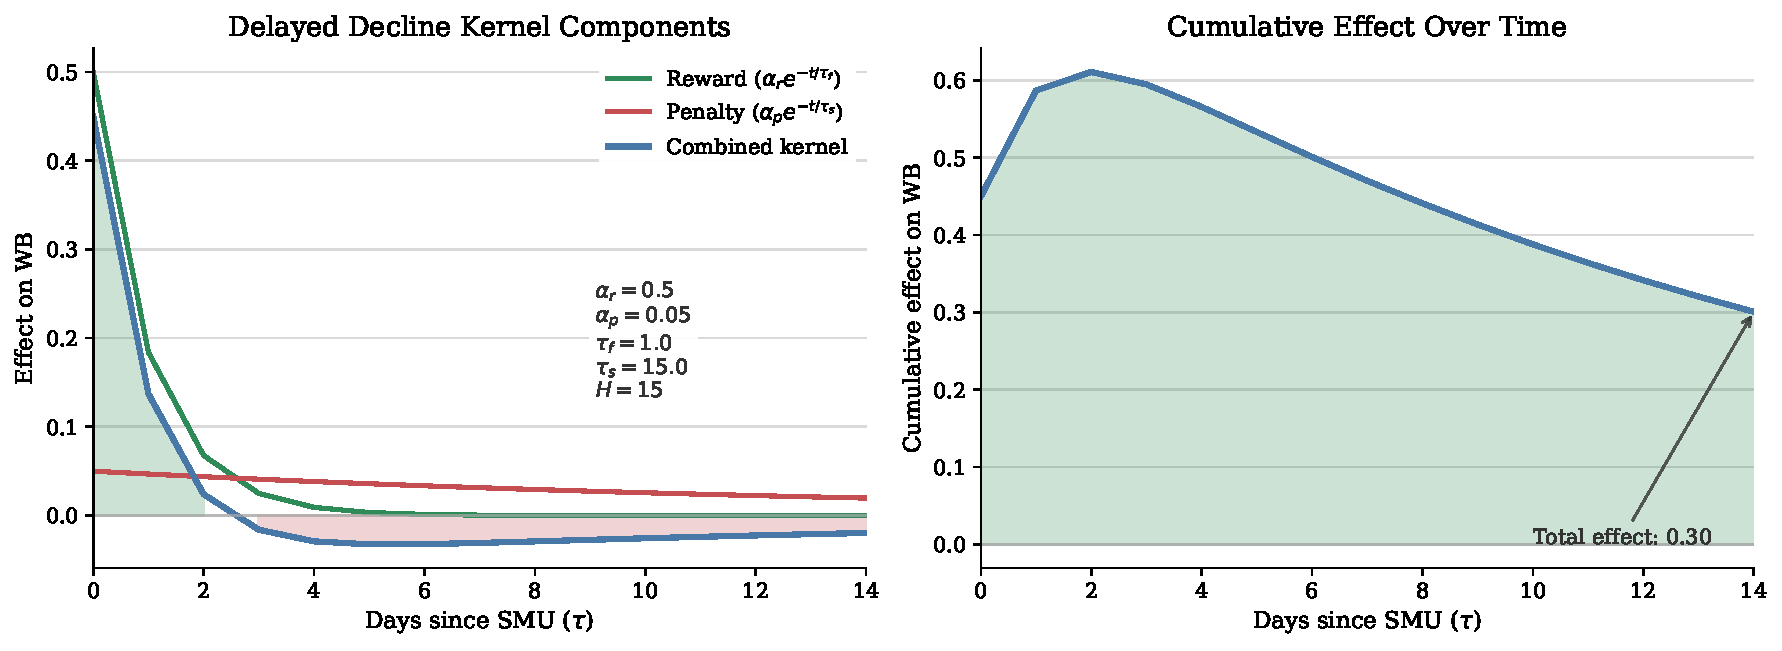
\includegraphics[width=\textwidth]{figures/delayed_decline_kernel.pdf}
    \caption[Delayed decline kernel used in the Simpson's Paradox simulation]{The delayed decline kernel used in the Simpson's Paradox simulation. The left panel shows the kernel effect, which is multiplied by each agent's SMU on the given day in the past. The green reward component declines rapidly due to $\tau_f = 1$, while the red penalty component declines slowly as $\tau_s = 15$. The red component is shown as positive here, but is subtracted from the green component in the blue combined kernel, which shows an immediate positive effect that quickly turns negative. The right panel shows the cumulative effect, assuming a constant unit of SMU over time. The kernel adds a positive cumulative effect, but the net effect after taking the direct effects of SMU and CoMO into account often becomes negative.}
    \label{fig:delayed_decline_kernel}
\end{figure}

To allow the delayed effects to have a clear influence at a population level, we use a larger population and more time steps than in the previous simulation. Additional parameter values are given in Appendix~\ref{app:code:abm}.

\subsection{Results and Interpretation}
\label{sec:abm:simpsons:results}
We visualise population mean SMU and WB throughout the simulation in Figure~\ref{fig:abm_simpsons_trends}. Here we see that after an initial volatile period (where the delayed effects kick in), the population moves to a decline in WB and increase in SMU\@.

\begin{figure}[htbp]
    \centering
    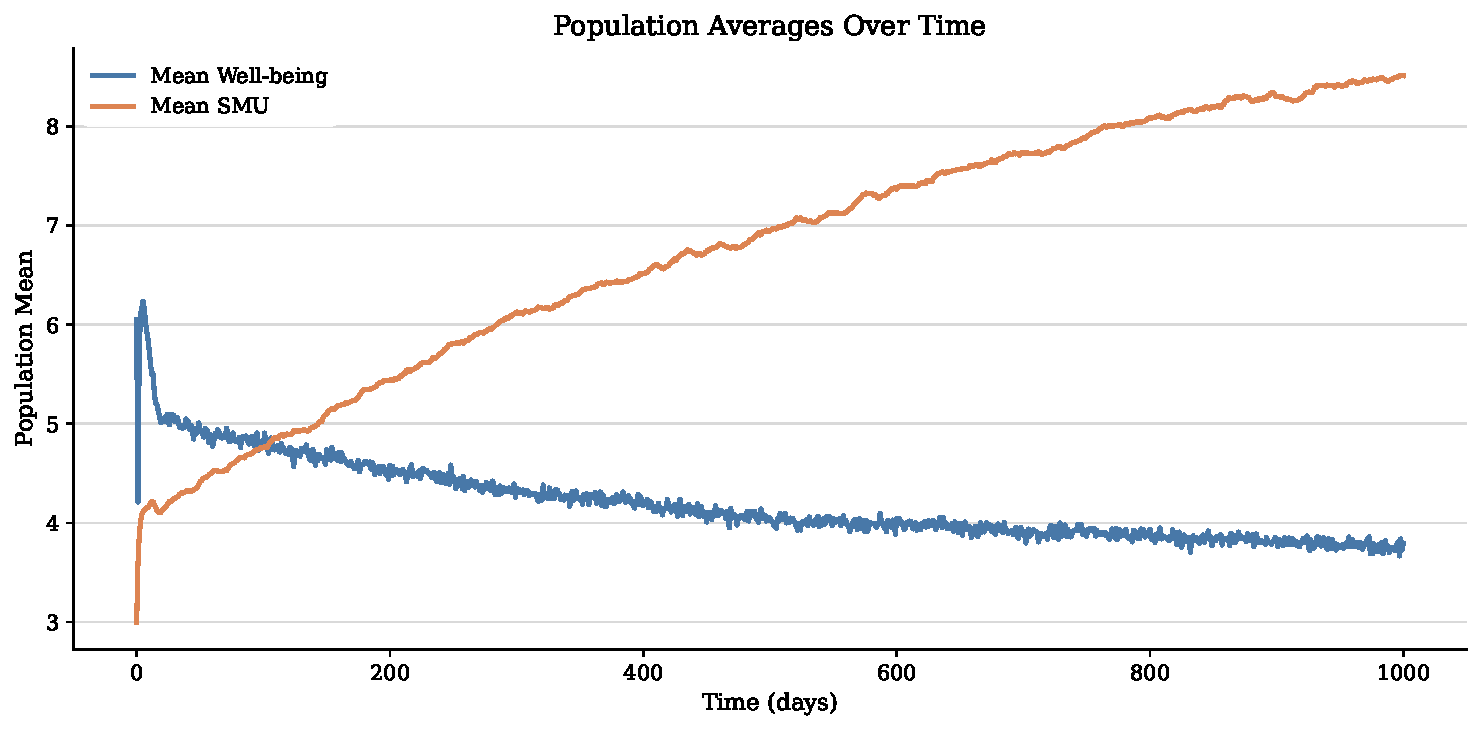
\includegraphics[width=\textwidth]{figures/abm_simpsons_trends.pdf}
    \caption[Average SMU and WB over time for the simulated population]{Average SMU and WB over time for the simulated population. The erratic start is caused by the delayed decline mechanism slowly kicking in.}
    \label{fig:abm_simpsons_trends}
\end{figure}

In Figure~\ref{fig:abm_simpsons_regressions} we visualise Simpson's Paradox. Here we again plot the mean WB of the population throughout the simulation period. We also show a scatter plot of the agents' SMU and WB values at times $t = 100$, $t = 500$, and $t = 900$, along with regression lines of simple linear regression using OLS\@. These all have positive slopes, showing how naive regression at any $t$ shows a different association than the one we observe at a population level.

\begin{figure}[htbp]
    \centering
    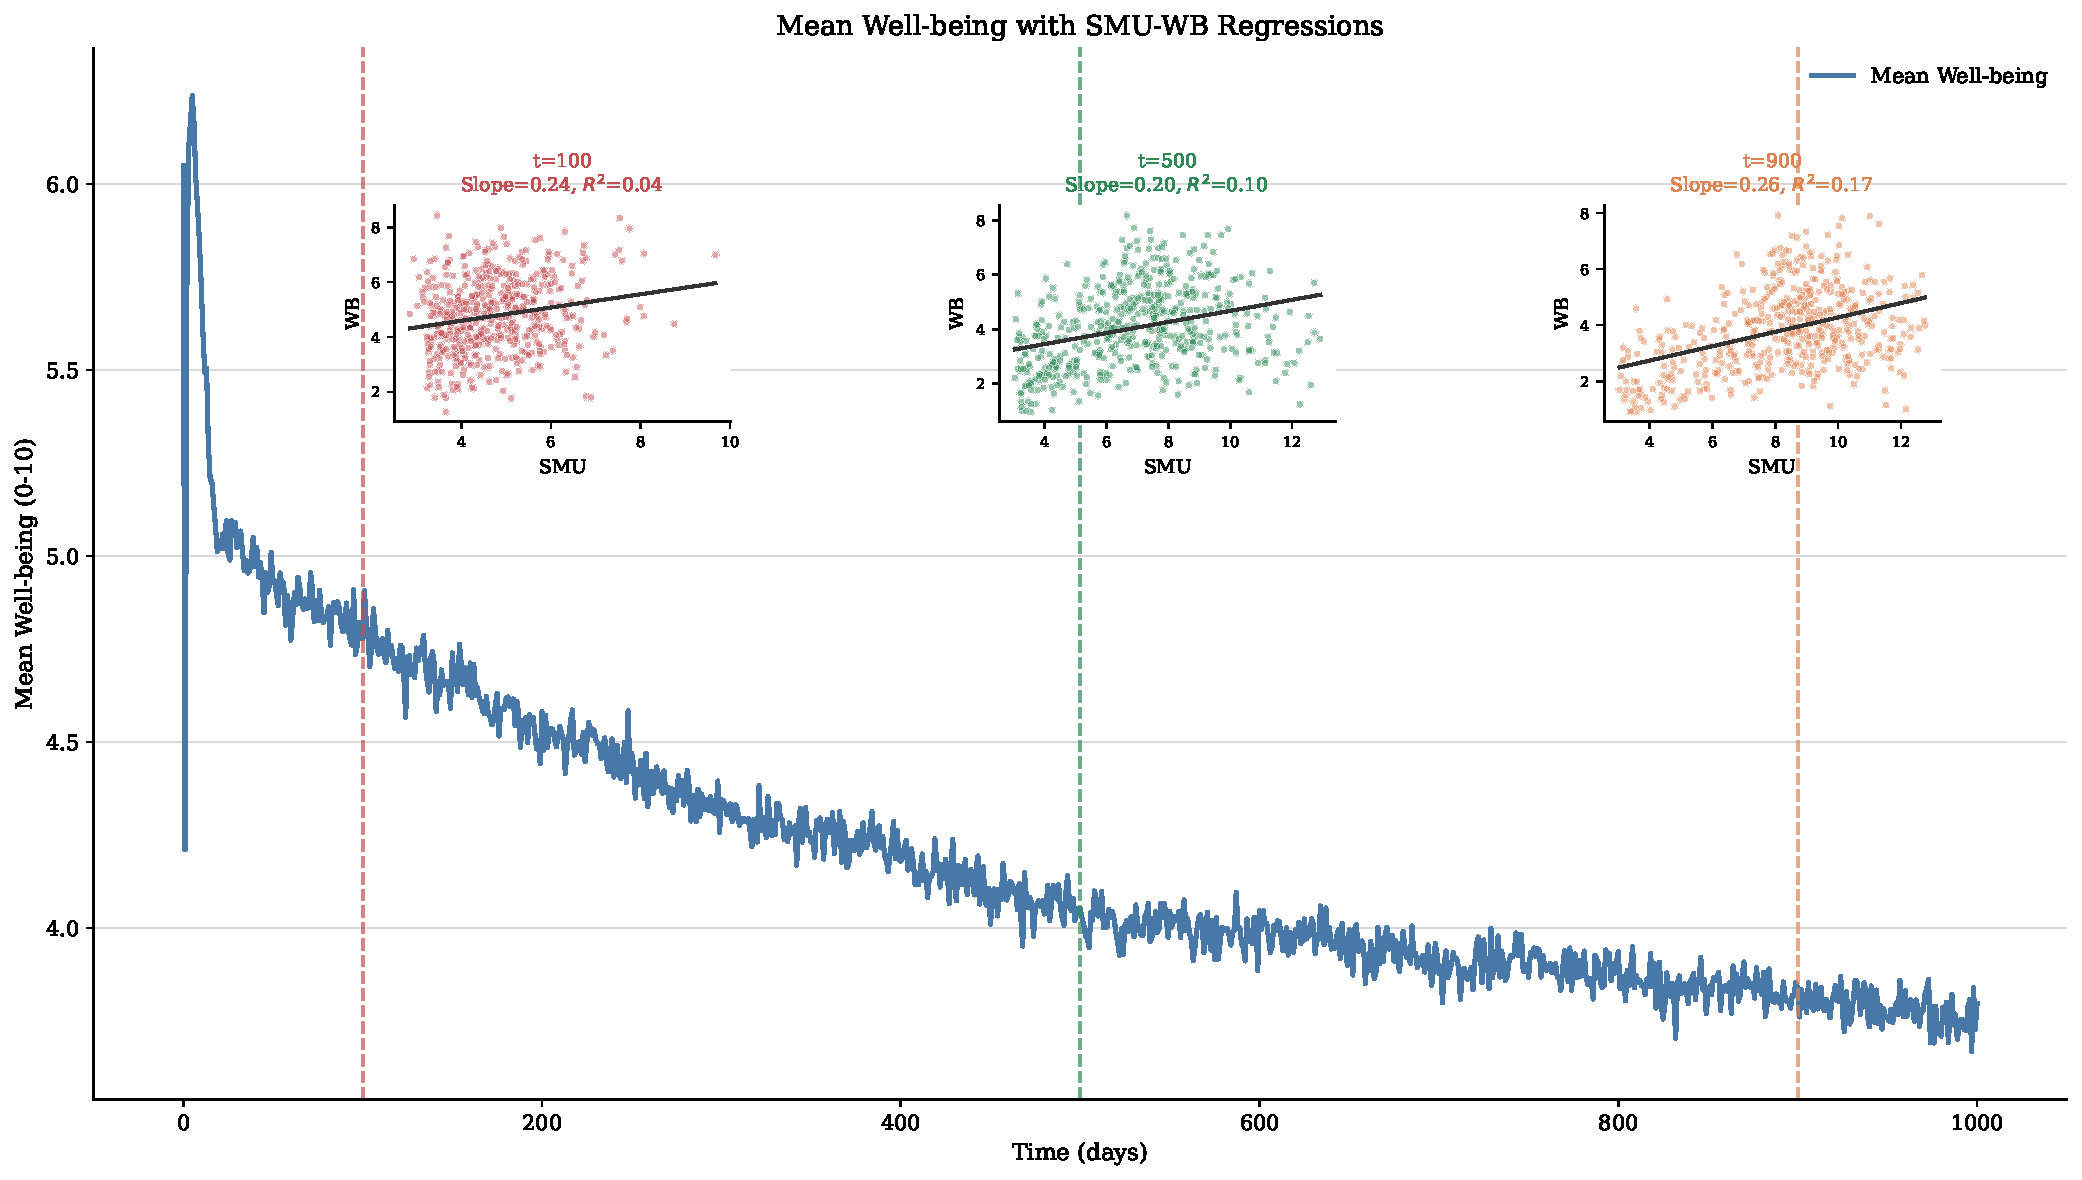
\includegraphics[width=\textwidth]{figures/abm_simpsons_regressions.pdf}
    \caption[Mean WB over time with cross-sectional SMU--WB regressions]{The blue line shows average WB over time for the simulated population. At $t = 100$, $500$, and $900$ we show scatter plots of all agents, with cross-sectional regression lines of the relationship between SMU and WB at each time point, all with positive slopes.}
    \label{fig:abm_simpsons_regressions}
\end{figure}

Hence, we see how the delayed decline mechanism combined with peer-comparison effects can lead to Simpson's Paradox. This implies a difficulty and a need to be very careful when interpreting results from the SMU--WB literature. From the point of view of a social scientist, we can imagine a researcher conducting a cross-sectional survey of a population at some time, finding a positive association between SMU and WB\@. From this, it would seem reasonable to conclude that SMU is harmless, or maybe even beneficial. Even a researcher who performed a longitudinal study, conducting multiple cross-sectional studies throughout time, would consistently find a positive association. However, as we can see when we look at the population-level trends, Simpson's Paradox is present, and the true causal effect is negative. Thus, we see that standard research methods might give very misleading results, and can even actively point in the opposite direction of the truth, when peer-comparison effects and temporal dynamics are present. This could have serious consequences when combined with large-scale policy implementations based on such findings.

In subsequent chapters we will focus on developing methods dealing with the bias shown in Section~\ref{sec:abm:results}.

%% Section 3.6: Discussion and Implications
\section{Discussion and Implications}
\label{sec:abm:implications}
Our simulation results showed biased estimates when the CoMO term and neighbour adjacency introduced network effects. We also showed how Simpson's Paradox led to further difficulties for causal interpretations. This section discusses the results with implications for the existing SMU--WB literature, and the path forward.

\subsection{Biased Results}

Why do we see biased results in our simulations? When we introduce the CoMO term with either population-level or neighbour-weighted social comparison, we are introducing network effects into our model, as well as an omitted regressor when it is not accounted for in the modelling.

The estimates made by cross-sectional OLS get biased because of violation of exogeneity in Assumption~\ref{ass:cross_sectional}. Here, CoMO will be an omitted regressor that is correlated with both SMU and WB\@.

For the OLS case, we can look formally at what is being calculated. The true DGP of our simulation is:

\begin{equation}
    y_i = \mu^y_i + \gamma_1 s_i + \gamma_2 \cdot c_i + \varepsilon_i
    \label{eq:ols_true_model_equation}
\end{equation}

The cross-sectional OLS regression estimates (omitting the CoMO variable):

\begin{equation}
y_i = \alpha + \tilde{\gamma}_1 s_i + u_i
\end{equation}

The OLS estimator is $\hat{\tilde{\gamma}}_1 = \frac{\Cov(s, y)}{\Var(s)}$. Substituting in the true model of Equation~\eqref{eq:ols_true_model_equation} for $y$ yields the standard omitted-variable bias formula \parencite[see][Eq.~(3.2.11), p.~60]{Angrist2009}, showing that $\hat{\tilde{\gamma}}_1$ converges in probability to:

\begin{equation}
\hat{\tilde{\gamma}}_1 \pto \gamma_1 + \gamma_2 \cdot \frac{\Cov(s, c)}{\Var(s)}
\end{equation}

For the CoMO term, agents with low SMU have higher values, so $\Cov(s, c) < 0$. As we also have $\gamma_2 < 0$, we get $\gamma_2 \cdot \frac{\Cov(s, c)}{\Var(s)} > 0$. As $\gamma_1$ is negative, this positive bias pulls it towards zero. This explains the bias towards zero, which is what we observe in our simulation results.

Assumption violations also lead to bias in the other two research methods. For the panel fixed effects we require uncorrelated errors and regressors across time in the strict exogeneity Assumption~\ref{ass:panel}. The network effects introduce time-varying confounding that cannot be controlled for by the fixed effects. The estimates made by RCTs rely on the SUTVA assumption (Assumption~\ref{ass:sutva}). When we cap SMU for the treatment group, this influences the reference level used in CoMO calculations for untreated agents as well. Hence, there is a spillover of the treatment into the control group, breaking the SUTVA assumption.

Mathematically, the SUTVA assumption translates into the RCT estimator $\hat{\tau} = \bar{y}^{\text{treated}} - \bar{y}^{\text{control}}$ being unbiased only when the outcomes of agents in the control group are unaffected by the treatment. However, when treated agents get their SMU reduced, this changes $\bar{s}^{\text{ref}}$ in the CoMO calculation for all agents (due to the network). Some of the outcome change of the treated group thus gets transferred to the control group, biasing $\hat{\tau}$ towards zero.

\subsection{Implications for Existing Literature}

As discussed in Section~\ref{sec:intro:motivation}, current research on SMU and WB has provided mixed results. We find it likely that network effects play a role. This has an important implication for the field of SMU--WB research in particular. Unlike other experimental fields, such as pharmaceutical trials, where patient outcomes are biologically independent (one patient taking a drug does not change drug efficacy in other patients), the individuals in SMU--WB research are involved in inherently networked systems. Thus, the SUTVA assumption underlying the gold standard of empirical research, RCTs, is violated. This leaves the field in a state where the causal question is still unanswered, which motivates the development of models taking network effects explicitly into account in subsequent chapters.

\subsection{Implications for Modelling of SMU--WB}

This chapter has shown that methods relying on individuals as independent units can be substantially biased when estimating causal effects in the presence of network effects. This motivates approaching the question through explicit modelling of network effects. In the next chapters, we will do just this. In Chapter~\ref{chap:model} we define a model for the influence of SMU on WB that explicitly includes network effects and the CoMO variable. In Chapters~\ref{chap:estimation} and~\ref{chap:monte_carlo} we use theory of maximum likelihood and two-stage least squares to find estimators for this model, and implement a Monte Carlo simulation study to validate the procedure. As we will see, under the assumption of our network-aware model, the estimators will produce unbiased estimates of the causal effects we are seeking. The model applies to a simpler DGP than the one used for our ABMs. In particular, it is static. Thus, we narrow the gap to ABMs without closing it. We discuss the remaining gap in Section~\ref{sec:discussion_conclusion:gap}.

